\section{Surrogate Models}
%-----------------------------------------------------------------------
%-----------------------------------------------------------------------
\begin{frame}[c]{Surrogate Models: Features}

\begin{columns}[T] % align columns
\begin{column}{.48\textwidth}
    \begin{block}{Mandatory}
    \begin{itemize}
    	\item<1-6> Regression model
    	\item<2-6> Uncertainty estimates
    	\item<3-6> Accurate predictions
    \end{itemize}
    \end{block}
    
    \only<4-6>{
        \begin{block}{Depending on the application}
        \begin{itemize}
        	\item<4-6> Cheap-to-train
        	\item<5-6> Scales with the complexity of the data
        	\note[item]{(number of features and observations)}
        	\item<6-6> Can handle different types of features
        	\note[item]{(categorical and continuous)}
        \end{itemize}
        \end{block}
    }
    
\end{column}%

\hfill%

\begin{column}{.48\textwidth}

\only<1-1>{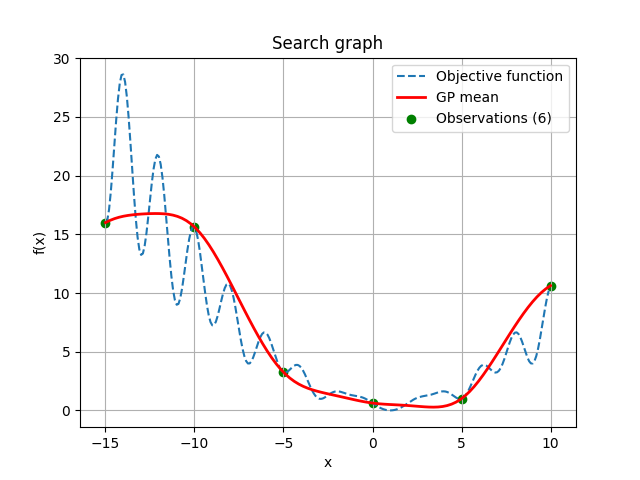
\includegraphics[width=1.\textwidth]{w06_hpo_bo/images/bo_loop_overview/03_mean.png}}
\only<2-6>{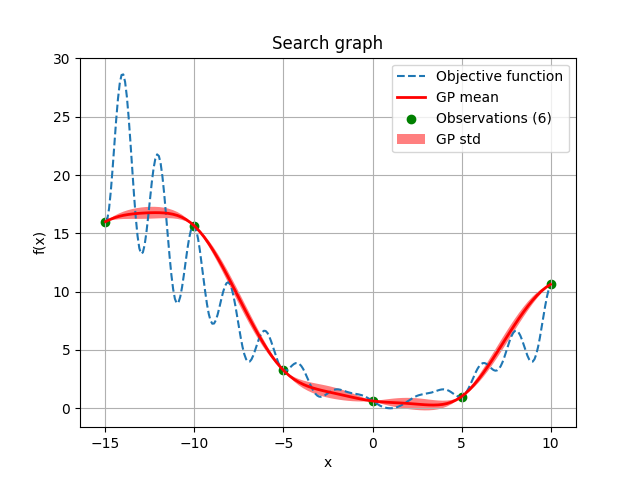
\includegraphics[width=1.\textwidth]{w06_hpo_bo/images/bo_loop_overview/04_std.png}}

\end{column}%
\end{columns}

\end{frame}
%-----------------------------------------------------------------------

%-----------------------------------------------------------------------
%-----------------------------------------------------------------------
\begin{frame}[c]{Surrogate Models: Candidates}

\begin{columns}[T] % align columns
\begin{column}{.48\textwidth}
\begin{itemize}
	\item<1-3> Gaussian Processes \note[item]{(quite common)}
	\item<2-3> Random Forests \note[item]{(our default choice)}
	\item<3-3> Bayesian Neural Networks \note[item]{(recent trend)}
\end{itemize}
\end{column}%

\hfill%

\begin{column}{.48\textwidth}
\only<1-1>{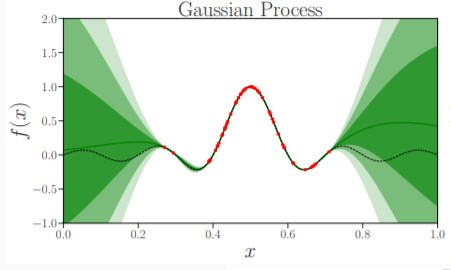
\includegraphics[width=1.\textwidth]{w06_hpo_bo/images/surrogate_models/uncertainty_gp.jpg}}
\only<2-2>{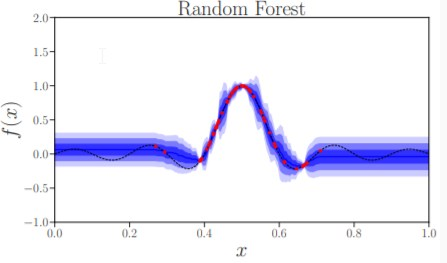
\includegraphics[width=1.\textwidth]{w06_hpo_bo/images/surrogate_models/uncertainty_forest.jpg}}
\only<3-3>{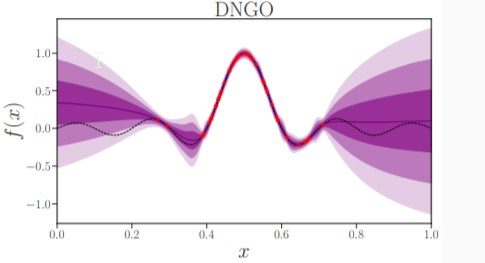
\includegraphics[width=1.\textwidth]{w06_hpo_bo/images/surrogate_models/uncertainty_dngo.jpg}}
\end{column}%
\end{columns}

\source{A. Klein: Introduction Automated Machine Learning}

\comment{adjust those plots}

\end{frame}
%-----------------------------------------------------------------------

%-----------------------------------------------------------------------
%-----------------------------------------------------------------------
\begin{frame}[c]{Surrogate Models: Gaussian Processes - reminder}

\begin{columns}[T] % align columns
\begin{column}{.48\textwidth}

\only<1-7>{
    \begin{block}{Advantages}
    \begin{itemize}
    	\item Smooth and reliable uncertainty estimates \pause
    	\item We can encode in the kernel expert knowledge about the design space \pause
    	\item ... 
    \end{itemize}
    \end{block}
}
\end{column}%

\hfill%

\begin{column}{.48\textwidth}
\only<3-7>{
    \begin{block}{Disadvantages}
    \begin{itemize}
    	\item We have to define a good kernel for each application \pause
    	\note[item]{(if we don't optimize small-dimensional, continuous functions)}
    	\item Cost scales cubically with the number of observations \pause
    	\note[item]{(because of inverting the kernel)}
    	\item Not easily applicable in discrete or conditional spaces \pause
    	\item Sensitive to its own hyperparameters
    \end{itemize}
\end{block}
}
\end{column}
\end{columns}

\note[item]{
	\begin{itemize}
		 \item e.g., special kernels for categorical hyperparameters and\\ conditional dependencies
	\end{itemize}
}
	
\note[item]{
    \begin{itemize}
    	\item to address this issue, there are sparse GPs\\ \lit{Snelson and Ghahramani. 2005}
    \end{itemize}
}

\end{frame}
%-----------------------------------------------------------------------

%-----------------------------------------------------------------------
%-----------------------------------------------------------------------
\begin{frame}[c]{Surrogate Models: Gaussian Processes - reminder}

\begin{itemize}
    \item<1-3> Samples from the prior are zero-mean, with values drawn from a multivariate Gaussian distribution
    \item<2-3> The kernel (covariance) function $K$ tells us how correlated the function values at two points are
    \item<3-3> The posterior is also a GP, with predictive distribution:
    \begin{equation*}
         P(\func_{\bocount+1} \vert \dataset_{1:\bocount}, \conf_{\bocount+1}) =  \mathcal{N}(\mean_{\bocount}(\conf_{\bocount+1}), \variance_{\bocount}(\conf_{\bocount+1}))
    \end{equation*}
    \begin{equation*}
        \mean_{\bocount}(\conf_{\bocount+1}) = \bm{k}^{T} \bm{K}^{-1} \bm{\func_{1:\bocount}}
    \end{equation*}
    \begin{equation*}
        \variance_{\bocount}(\conf_{\bocount+1}) = k(\conf_{\bocount+1}, \conf_{\bocount+1}) - \bm{k}^{T} \bm{K}^{-1} \bm{k}
    \end{equation*}
\end{itemize}


\note[item]{for the review of GPs - Rasmussen and Williams}

\end{frame}
%-----------------------------------------------------------------------
 
%-----------------------------------------------------------------------
%-----------------------------------------------------------------------
\begin{frame}[c]{Surrogate Models: GPs - kernel hyperparameters}

\begin{itemize}
    \item After choosing the kernel, we must also manage the hyperparameters that govern its behaviour, as well as that of the mean function.  \pause
    \item For our problems of interest, typically we have $D + 3$ GPs hyperparameters:  \pause
    \begin{itemize}
        \item $D$ length scales $\theta_{1:D}$, \pause
        \item the covariance amplitude $\theta_{0}$, \pause
        \item the observation noise $\noise$, \pause
        \item a constant mean $\mean$. 
    \end{itemize}
\end{itemize}

\end{frame}
%-----------------------------------------------------------------------

%-----------------------------------------------------------------------
%-----------------------------------------------------------------------
\begin{frame}[c]{Surrogate Models: GPs - kernel hyperparameters}

\begin{columns}[T] % align columns
\begin{column}{.58\textwidth}
\begin{itemize}
    \item We can use Maximum A Posteriori (MAP) or Maximum Likelihood Estimation (MLE) to sample hyperparameters \pause
    \item However, it is more realistic not to assume that hyperparameters distribution can be represented by a single point
\end{itemize}
\end{column}%

\hfill%

\begin{column}{.38\textwidth}
\end{column}%
\end{columns}

\source{Snoek et al. 2015}
\end{frame}
%-----------------------------------------------------------------------

%-----------------------------------------------------------------------
%-----------------------------------------------------------------------
\begin{frame}[c]{Surrogate Models: GPs - kernel hyperparameters}

\begin{columns}[T] % align columns
\begin{column}{.58\textwidth}
\begin{itemize}
    \item<1-4> Markov-Chain Monte-Carlo (MCMC) drops this assumption and samples hyperparameters from a distribution proportional to their probability, given the data and prior assumptions
    \item<2-4> Marginalize over hyperparameters and compute integrated acquisition function:
        \begin{equation*}
        \begin{aligned}
            \hat{\acq} ( \conf; \left \{ \bonextsample, \bonextobs \right \} ) = \int \acq ( \conf; \left \{ \bonextsample, \bonextobs \right \}, \theta ) \\ 
            p(\theta  \rvert \left \{ \bonextsample, \bonextobs \right \}^{\bobudget}_{\bocount=1} )d\theta
        \end{aligned}
        \end{equation*}
    \item<3-4> MCMC is more computationally expensive than gradient based optimization
    \item<4-4>The acquisition function must now be calculated more than just once
\end{itemize}
\end{column}%

\hfill%

\begin{column}{.38\textwidth}
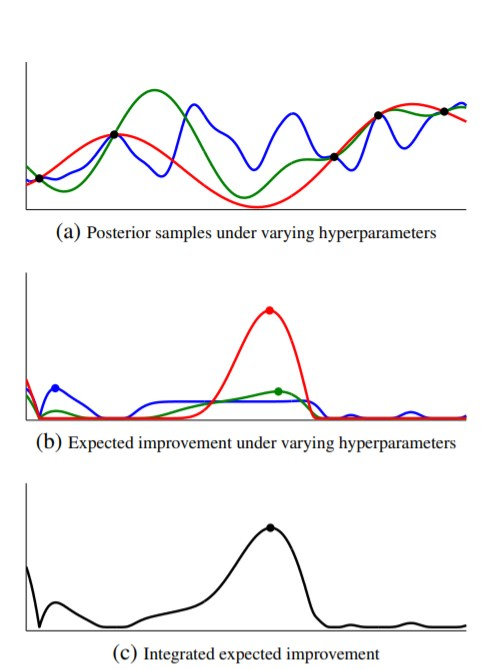
\includegraphics[width=0.9\textwidth]{w06_hpo_bo/images/surrogate_models/kernel_hp_mcmc.jpg}
\end{column}%
\end{columns}

\source{Snoek et al. 2015}
\end{frame}
%-----------------------------------------------------------------------

%-----------------------------------------------------------------------
%-----------------------------------------------------------------------
\begin{frame}[c]{Surrogate Models: Random Forests}

\begin{columns}[T] % align columns
\begin{column}{.48\textwidth}


\begin{block}{Train}
\begin{itemize}
	\item<1-6> $n$ regression trees. 
	\item<2-6> Subsampled training data for each tree (with bootstrapping).
	\item<3-6> Each tree gives us a possible explanation for the observations.
\end{itemize}
\end{block}

\only<4-6>{
    \begin{block}{Predict}
    \begin{itemize}
    	\item<4-6> Obtain prediction of each tree.
    	\item<5-6> Aggregate predictions (e.g., average).
    	\item<6-6> Uncertainty of predictions: stdev across tree predictions. 
    \end{itemize}
    \end{block}
}
\end{column}%

\note[item]{Uncertainty in the leaves is dropped}

\hfill%

\begin{column}{.48\textwidth}
\only<1-6>{
    \centering
    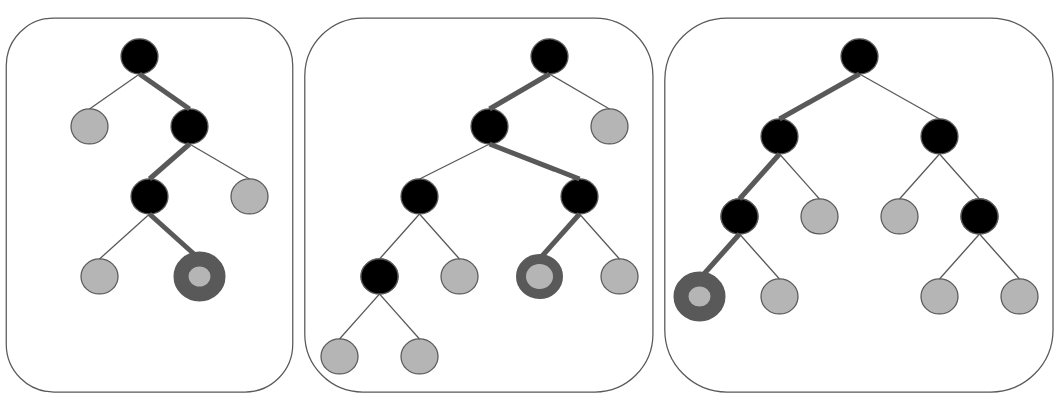
\includegraphics[width=0.8\textwidth]{images/surrogate_models/random_forest_pic}
}
\end{column}
\end{columns}

\end{frame}
%-----------------------------------------------------------------------

%-----------------------------------------------------------------------
%-----------------------------------------------------------------------
\begin{frame}[c]{Surrogate Models: Random Forests - hyperparameters}

\begin{columns}
	\column{0.5\textwidth}
	\centering
	w bootstrapping and\\ w/o random splits
	
	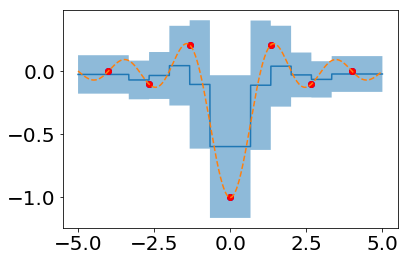
\includegraphics[width=0.6\textwidth]{images/surrogate_models/rf_boot_middle_split.png}
	
	
	w bootstrapping and\\ w/ random splits
	
	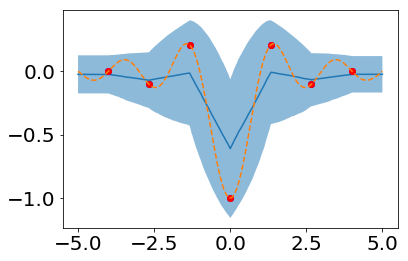
\includegraphics[width=0.6\textwidth]{images/surrogate_models/rf_boot_rand_split.png}

	\column{0.5\textwidth}
	\centering
	w/o bootstrapping and\\ w/o random splits
	
	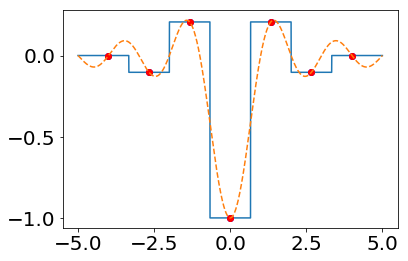
\includegraphics[width=0.6\textwidth]{images/surrogate_models/rf_noboot_middle_split.png}
	
	w/o bootstrapping and\\ w/ random splits
	
	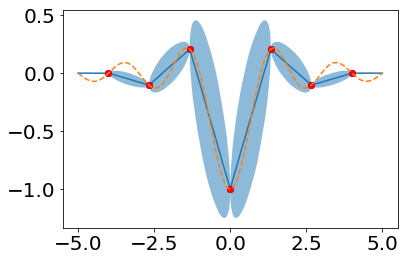
\includegraphics[width=0.6\textwidth]{images/surrogate_models/rf_noboot_rand_split.png}
	
\end{columns}

\end{frame}
%-----------------------------------------------------------------------

%-----------------------------------------------------------------------
%-----------------------------------------------------------------------
\begin{frame}[c]{Surrogate Models: Random Forests - summary}


\begin{columns}[T] % align columns
\begin{column}{.48\textwidth}

\only<1-8>{
    \begin{block}{Advantages}
    \begin{itemize}
        \item Cheap to train \pause
        \item Scales well with \#observations: 
        \begin{itemize}
        	\item Worst-case complexity for $T$ tress with $n$ data points of dimensionality $p$: $\mathcal O(T\cdot p \cdot n^2 \log{n})$. \pause
        \end{itemize}
        \item Training can be parallelized \pause
        \item Can easily handle conditional, categorical, continuous and discrete spaces \pause
        \item Fairly robust against its own hyperparameters
    \end{itemize}
    \end{block}
}
\end{column}%

\hfill%
\pause

\begin{column}{.48\textwidth}
\only<6-8>{
    \begin{block}{Disadvantages}
    \begin{itemize}
        \item Poor uncertainty estimates \pause
        \item Poor extrapolation (constant) \pause
    	\item Priors cannot easily be incorporated
    \end{itemize}
    \end{block}
}
\end{column}
\end{columns}

\end{frame}
%-----------------------------------------------------------------------

%-----------------------------------------------------------------------
%-----------------------------------------------------------------------
\begin{frame}[c]{Surrogate Models: Bayesian Neural Networks - Idea}

\begin{itemize}
    \item Deal with all sources of parameter uncertainty: \pause
    \begin{itemize}
        \item More than one weight vector can explain the observed data 
        \item Take into account all possible explanations 
    \end{itemize}

\centering
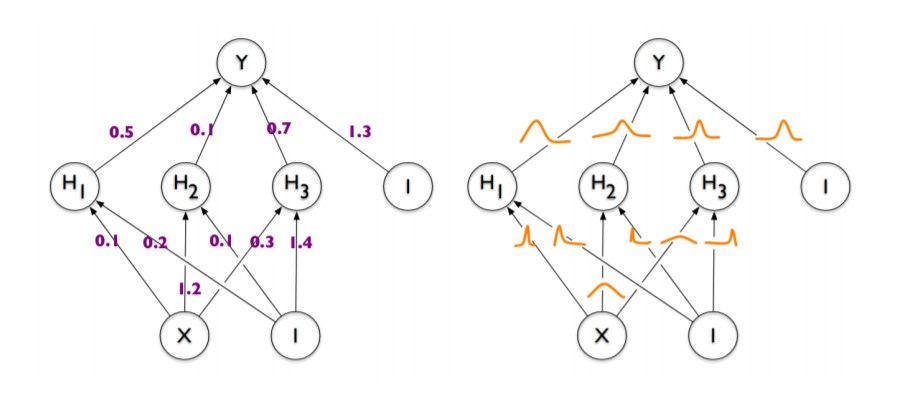
\includegraphics[width=0.6\textwidth]{w06_hpo_bo/images/surrogate_models/bnn.jpg}

\end{itemize}

\source{Blundell et al.: Weight Uncertainty in Neural Networks}

\end{frame}
%-----------------------------------------------------------------------

%-----------------------------------------------------------------------
%-----------------------------------------------------------------------
\begin{frame}[c]{Surrogate Models: Bayesian Neural Networks - Idea}

\begin{itemize}
    \item Deal with all sources of parameter uncertainty
    \item If possible, also deal with all sources of architecture uncertainty \pause
     \begin{itemize}
        \item This would mean not to determine a single architecture, but a
distribution \pause
        \item For every architecture, one would still want to be Bayesian about its weights... \pause
        \item Nobody is really Bayesian about architectures these days \pause
        \item This has been too expensive; but that may change with efficient
gradient-based architecture search methods...
    \end{itemize}
\end{itemize}

\end{frame}
%-----------------------------------------------------------------------


%-----------------------------------------------------------------------
%-----------------------------------------------------------------------
\begin{frame}[c]{Surrogate Models: BNNs for Bayesian optimization}

\begin{itemize}
	\item BNNs are known to have good predictions given big data \pause
	\item In Bayesian optimization, we have (often) little data \pause
	\item Nevertheless, we can use BNNs for BO \pause
	\bigskip
	\item Different implementations:
	\begin{itemize}
	    \item Snoek et al.: Scalable Bayesian Optimization Using Deep Neural Networks, \pause
	    \item Springenberg et al.: Bayesian Optimization with Robust Bayesian Neural Networks, \pause
        \item Schilling et al.: Hyperparameter Optimization with Factorized Multilayer Perceptrons, \pause
        \item Perrone et al.: Scalable Hyperparameter Transfer Learning, \pause
        \item Hern\'andez-Lobato et al.: Parallel and Distributed Thompson Sampling for Large-scale Accelerated Exploration of Chemical Space.

	\end{itemize}
\end{itemize}

\end{frame}
%-----------------------------------------------------------------------

%-----------------------------------------------------------------------
%-----------------------------------------------------------------------
\begin{frame}[c]{Surrogate Models: Bayesian Neural Networks - DNGO}

\begin{itemize}
    \item Fit a standard neural network to the data \pause
    \item Use the representation in the last hidden layer as basis \\ functions $\phi(x)$ of the input $x$ \pause
    \item Use Bayesian linear regression for the output layer
    \begin{itemize}
        \item The last layer is linear in its parameters $\theta$  \pause
        \item Therefore, the Bayesian linear regression formulas work directly \pause
        \item Feasible in closed form, in time $O(N d^3)$, \\ where $N$ is the number of data points and $d$ is the number of \\ hidden units in the last layer \pause
    \end{itemize}
    
\end{itemize}

\end{frame}
%-----------------------------------------------------------------------

%-----------------------------------------------------------------------
%-----------------------------------------------------------------------
\begin{frame}[c]{Surrogate Models: DNGO - summary}


\begin{columns}[T] % align columns
\begin{column}{.48\textwidth}

\only<1-7>{
    \begin{block}{Advantages}
    \begin{itemize}
        \item Scales linearly with \#observations \pause
        \item Given enough network samples obtain nice and smooth uncertainty estimates \pause
        \item Can handle categorical, continuous and discrete spaces
    \end{itemize}
    \end{block}
}
\end{column}%

\hfill%
\pause

\begin{column}{.48\textwidth}
\only<4-7>{
    \begin{block}{Disadvantages}
    \begin{itemize}
        \item Poor uncertainty estimates \pause
        \item Many meta-design decisions \pause
    	\item No follow-up research \pause
    	\item Need usually more data than Gaussian processes
    \end{itemize}
    \end{block}
}
\end{column}
\end{columns}

\end{frame}
%-----------------------------------------------------------------------
